\documentclass[12pt,a4paper,twocolumn]{article}
\usepackage[utf8]{inputenc}
\usepackage{amsmath}
\usepackage{amsfonts}
\usepackage{amssymb}
\usepackage{graphicx}
\usepackage{authblk}
\usepackage[font=small,labelfont=bf]{caption}

\title{``How Prolific Are You?": A Scientometric Analysis of Researchers}

\author[1]{Rahul Yedida}
\author[2]{Adel Aladwani}
\author[1]{Snehanshu Saha}
\affil[1]{Department of Computer Science \& Engineering, PES University}
\affil[2]{Department of Information Systems, Kuwait University}

\date{}
\begin{document}
	\maketitle
	
	\abstract{
		Scholars in academia regularly write papers showing the results of their work. To gauge how relevant their work is, several measures are used, including citation count and the h-index. This paper describes the methods used to identify ``prolific" authors, whose metrics are significantly higher than their peers, and provides a general discussion of the relationships between different metrics. We also discuss how this analysis is performed even with the high dimensionality of the dataset.
	}
	
	\section{Introduction}
	Scientometrics is the study of measuring science and research. Several measures are currently in use to measure the output of researchers, and each of these individually may not be an indicator of the quality and repute of a scholar's work. Comparing researchers by several metrics at once is cumbersome to do manually, and it would be incorrect to use a function of several metrics to compare how ``prolific" a researcher is. In this paper, we first identify linear relationships among the attributes. We assert that this is also useful in finding the ``most important" features. Later, we use two algorithms to cluster the records and compare the outputs of both algorithms. Finally, we use these results to identify prolific authors. 
	
	The rest of the paper is structured as follows. Section 2 describes the data and shows correlations between the attributes. Section 3 discusses the methods we used to analyse this data.
	
	\section{Data}
	The data contains 618 records of scholars with 25 attributes. There are no missing values, and eight of the attributes are integers. For ease of analysis, we have labeled the attributes as \textit{v1} through \textit{v25}. A table explaining what each of these variables are is given in Table 1 of the Supplementary Materials section at the end of this paper.
	
	\subsection{Preliminary Analysis}
	For a preliminary analysis of the relationships between the attributes, we sought to discover monotonic relationships. This was done by computing pairwise Spearman's rank correlation coefficient. This revealed that there were only positive monotonic relationships. 42.08\% of these coefficients were above 0.8, and 52\% were above 0.7.
	
	A logical next step, then, was to investigate the percentage of linear relationships among these. This was done by computing pairwise Pearson correlation coefficients. To visually understand pairs that had high linear correlations, we displayed this information in a matrix, maintaining only the upper half, and avoiding diagonal entries. This avoids counting self-correlations and counting the same pair twice. Further, when finding multiple linear regression equations, this finds only unique relations between the variables. Figure 1 shows this result. Asterisks indicate a Pearson R value of 0.8 or higher. The numbers at the right indicate how many other variables each variable is highly correlated with. \\
	
	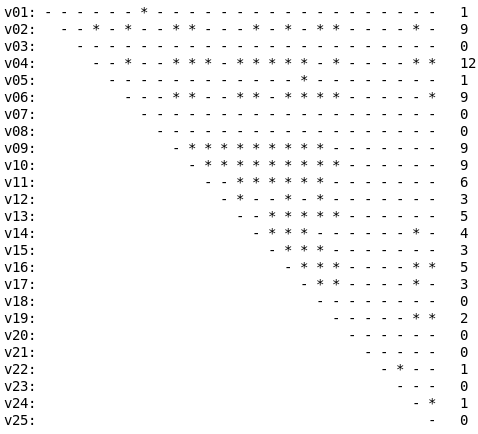
\includegraphics[scale=0.4]{fig1.png}
	\begingroup
	\captionof{figure}{Matrix showing pairs with Pearson R values 0.8 or higher}
	\endgroup
	\hfill\break
	These correlations provide a starting point to find relationships between the attributes.
	
	\section{Methods}
	This section discusses in detail the methods used to analyse the data.
	
	\subsection{Regression Analysis}
	Our first analysis investigated the precise relationships between the attributes. We looked at linear relationships. Because v4 had the most number of correlations, we started with it.
	
	Multiple regression analysis was performed as follows. For each attribute that the variable being analysed has a high correlation with, we ran an Ordinary Least Squares (OLS) regression model in two cases--with a constant term and without (that is, in a forward step-wise fashion). 
	
	In each case, for each variable, we check the p-value to ensure that all variables are statistically significant. Finally, we choose the model with the highest adjusted $R^2$ value, which avoids the pitfalls of ``kitchen sink regression". We also make sure that there are no significant autocorrelations, using the Durbin-Watson test. \cite{field2009discovering} suggests that a conservative range for the acceptable values for this test is between 1 and 3. In some cases, we chose to pick a model that has a slightly lesser adjusted $R^2$ value in favor of using lesser variables. This results in a model that still has a high predictive power, yet is simpler. In addition, we also check the residuals vs. fits plots and check that they are not very correlated. 
	
	We note here that this analysis may be useful for identifying ``important" attributes in a dataset. If a model that predicts a dependent variable through the other attributes yields a high adjusted $R^2$ value, then we may safely remove this dependent variable, keeping only the statistically significant predictor variables from the regression analysis.
	
	The full regression results can be found in the Supplementary Materials section at the end of this paper. Here, we present a summary of the results of the regression analysis that was performed.
	
	\subsubsection{Analysis on the full data}
	We first looked at v4, and did a step-wise regression analysis. \textit{v6, v9, v11, v13, v14, v17, v19, v24,} and \textit{v25} were statistically significant, and the adjusted $R^2$ was 0.972. For this model, the Durbin-Watson statistic was 2.06, which suggests very minor negative autocorrelations. The correlations between the residuals and the fitted values was -0.0047. Figure 2 shows the residuals vs. fits plot for \textit{v4}.\\
	
	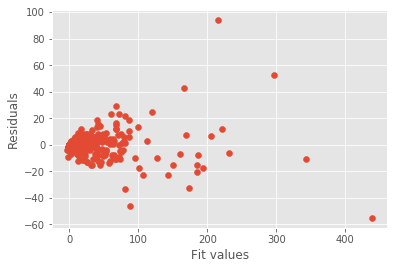
\includegraphics[scale=0.5]{fig2.png}
	\begingroup
	\captionof{figure}{Residuals vs. fits plot for v4}
	\endgroup
	\hfill\break
	
	Our next variable of interest was \textit{v2}, having high Pearson R correlations with nine other variables. Only \textit{v9} was not statistically significant. However, we also chose to discard \textit{v24} because it added no predictive power to the model, and the adjusted $R^2$ for this model was 0.993, and the Durbin-Watson statistic was 1.853, suggesting only minor positive autocorrelations. All the p-values were less than $10^{-3}$. The correlation between the residuals and the fits was 0.023. Figure 3 shows the residuals vs. fits plot for \textit{v2}.
	
	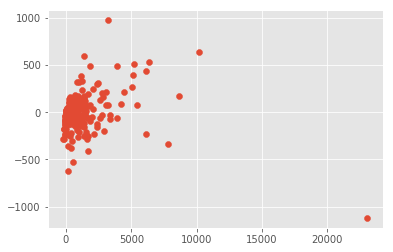
\includegraphics[scale=0.5]{fig3.png}
	\begingroup
	\captionof{figure}{Residuals vs. fits plot for v2}
	\endgroup
	\hfill\break
	
	We then looked at \textit{v6}, also having high correlations with nine other variables. \textit{v9} and \textit{v14} were not statistically significant. We also discarded \textit{v25} to obtain a simpler model with an adjusted $R^2$ value 0.001 less. This model had an adjusted $R^2$ of 0.913, and a Durbin-Watson statistic of 1.64. All p-values were below $10^{-3}$.
	
	Next, we looked at \textit{v9}. Only \textit{v13} was not statistically significant, but we also discarded \textit{v10} and \textit{v11}, which resulted in a model whose adjusted $R^2$ was 0.986 (a reduction of 0.002 from when the two variables were included). This model had a Durbin-Watson statistic of 1.99.
	
	Finally, for \textit{v10}, all the predictor variables were statistically significant, and we discarded \textit{v19}, which resulted in a model with the same adjusted $R^2$. All the p-values were below $10^{-3}$, except \textit{v13}, whose p-value was 0.043 (95\% C.I [0.07, 0.425]). The Durbin-Watson statistic was 1.861.
	
	It should be noted that in all of the regression results of the above variables, the constant was not statistically significant, and the results reported are those for the models that did not include the constant.
	
	\subsubsection{Analysis on subset of the data}
	Our next step of analysis was to pick a subset of the variables, and redo the same analysis discussed above on this subset. Once again, it turns out that for all the regression equations obtained, the constant was not statistically significant.
	
	The variables we chose were \textit{v9} through \textit{v21} and \textit{v24}. Again, we created a matrix of Pearson R correlations, and picked out those that were higher than 0.8. Figure 4 shows this result. \\
	
	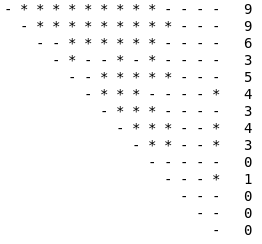
\includegraphics[scale=0.6]{fig4.png}
	\begingroup
	\captionof{figure}{Pearson R correlation matrix for subset of the data}
	\endgroup
	\hfill\break
	
	Using this, we redid the same analysis as in the previous subsection. Again, we only discuss the results here, but the full list of experiments is in the Supplementary Materials section.
	
	We first looked at v9. \textit{v13} was not significant when all the variables it was correlated to were considered. However, when \textit{v10} was not considered, it was statistically significant. We chose to sacrifice 0.2\% adjusted $R^2$ in favor of a model that had two fewer predictor variables. The Durbin-Watson value was 1.99.
	
	While predicting \textit{v10}, dropping \textit{v19} resulted in no loss of adjusted $R^2$. We further dropped \textit{v18}, and dropped \textit{v12} because it was not significant. While dropping \textit{v18} caused a 0.3\% drop in adjusted $R^2$, we were able to use two less variables. The Durbin-Watson statistic was 1.991.
	
	We only looked at two other variables, because the adjusted $R^2$ for the others was below 0.95. For \textit{v11}, dropping \textit{v17} and \textit{v18} resulted in a 0.2\% drop in adjusted $R^2$, and we were able to use only four variables to get an adjusted $R^2$ of 0.971 and a Durbin-Watson of 2.081. Finally, for \textit{v13}, all variables were statistically significant, and we discarded \textit{v19} with no loss of adjusted $R^2$.
	
	Perhaps more interesting than the above results was when we plotted the maximum adjusted $R^2$ (without discarding any variables) against the number of predictor variables used (on this subset of the data). Figure 5 shows this result, where a logarithm function fits quite well to the data. This meets our intuition of ``diminishing returns" as we increase the number of predictor variables. The equation obtained was
	\begin{equation}
	\text{Adj. } R^2 = 0.125465 \log n + 0.746654
	\end{equation}
	
	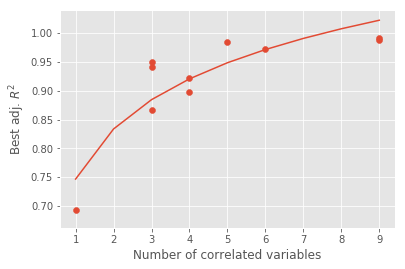
\includegraphics[scale=0.5]{fig5.png}
	\begingroup
	\captionof{figure}{Adjusted $R^2$ vs. number of predictor variables}
	\endgroup
	\hfill\break
	
	The sum of the squared residuals for this fit was 0.01456.
	
	\subsection{Cluster Analysis}
	We next sought to cluster the points, as a first step towards identifying ``prolific" authors. Because finding the number of clusters in such high dimensional data is difficult, we chose to use two different algorithms--DBSCAN (Density-Based Spatial Clustering of Applications with Noise)\cite{ester1996density} and mean-shift clustering \cite{comaniciu2002mean} from Python's sklearn package \cite{scikit-learn}. We picked two subsets of the data to perform this analysis on--the first was the set of variables that were highly correlated with \textit{v4} (denote this subset as $S_1$)--we chose these because it had an especially high number of correlated variables--and the second was the subset discussed in the previous subsection (which we shall denote as $S_2$. We also performed the clustering analysis with DBSCAN using PCA instead of manually picking features. The results of that are discussed in the Supplementary Materials.
	
	Because DBSCAN requires an \textit{eps} parameter, we chose to find a reasonable guess. We did this by setting a threshold that no more than roughly 10\% of the points (we chose 60 points) should be in individual custers. We started with an initial \textit{eps} guess of 0.5 and made increments of 0.1 till this condition was satisfied.
	
	We did not scale the features before clustering, because the distributions of all the features were different (running a Kolgomorov-Smirnov test on every pair of features gave p-values < 0.05). To prove that feature scaling is an incorrect step empirically, we performed both z-standardization and feature scaling to [0, 100]. In both cases, we found the value of \textit{eps} in the same way discussed above, but starting from 0.001 and going in increments of 0.001. In both cases, DBSCAN returned 60 individual clusters, and one other cluster containing all the points.
	
	For $S_1$, the value of \textit{eps} we arrived at was 45. Apart from 60 individual clusters, the algorithm identified three clusters of points. The results of this are summarized in Table 1. \\
	
	\begin{tabular}{|c|c|}
		\hline 
		\textbf{Cluster} & \textbf{Number of points} \\ 
		\hline 
		-1 & 60 \\ 
		\hline 
		0 & 532 \\ 
		\hline 
		1 & 20 \\ 
		\hline 
		2 & 6 \\ 
		\hline 
	\end{tabular}
	\begingroup
	\captionof{table}{DBSCAN clustering results on $S_1$}
	\endgroup
	\hfill\break
	
	The cluster -1 represents individual clusters. The rest of the clusters were arbitrarily numbered from zero. Next, we ran mean-shift clustering, which automatically finds clusters by estimating a \textit{bandwidth} parameter. Mean-Shift clustering identified 12 clusters, out of which five were individual clusters. We summarize these results in Table 2.\\
	
	\begin{tabular}{|c|c|}
		\hline 
		\textbf{Cluster} & \textbf{Number of points} \\ 
		\hline 
		-1 & 5 \\ 
		\hline 
		0 & 509 \\ 
		\hline 
		1 & 72 \\ 
		\hline 
		2 & 19 \\ 
		\hline 
		3 & 4 \\ 
		\hline 
		4 & 4 \\ 
		\hline 
		5 & 3 \\ 
		\hline 
		6 & 2 \\ 
		\hline 
	\end{tabular}
	\begingroup
	\captionof{table}{Mean-Shift clustering results for $S_1$}
	\endgroup
	\hfill\break
	
	We then checked whether the points in similar-sized clusters in each algorithm were the same. We briefly do this analysis for $S_1$, but conduct a more thorough investigation for $S_2$.
	
	We first looked at cluster 0 of both algorithms. Of these, 507 points were common, indicating that the majority of the dataset was clustered into the same cluster by both algorithms. Interestingly, however, this seems to be the only major commonality between the outputs of these algorithms. For example, cluster 1 of DBSCAN and cluster 2 of Mean-Shift, which had a very similar number of points, had no common points at all. Finally, 21 of the points that were marked as individual clusters by DBSCAN were put into cluster 1 by Mean-Shift.
	
	Next, we performed the above analysis for $S_2$. The value of \textit{eps} we arrived at was 18.6, and DBSCAN identified three clusters apart from sixty individual clusters. A summary is provided in Table 3, again, with cluster -1 meaning individual clusters.\\
	
	\begin{tabular}{|c|c|}
		\hline 
		\textbf{Cluster} & \textbf{Number of points} \\ 
		\hline 
		-1 & 60 \\ 
		\hline 
		0 & 541 \\ 
		\hline 
		1 & 3 \\ 
		\hline 
		2 & 14 \\ 
		\hline 
	\end{tabular} 
	\begingroup
	\captionof{table}{DBSCAN clustering results for $S_2$}
	\endgroup
	\hfill\break
	
	Table 4 summarizes the results of mean-shift clustering, which identified seven ``real" clusters and eight individual clusters.\\
	
	\begin{tabular}{|c|c|}
		\hline 
		\textbf{Cluster} & \textbf{Number of points} \\ 
		\hline 
		-1 & 8 \\ 
		\hline 
		0 & 504 \\ 
		\hline 
		1 & 82 \\ 
		\hline 
		2 & 15 \\ 
		\hline 
		3 & 3 \\ 
		\hline 
		4 & 2 \\ 
		\hline 
		5 & 2 \\ 
		\hline 
		6 & 2 \\ 
		\hline 
	\end{tabular} 
	\begingroup
	\captionof{table}{Mean-Shift clustering results for $S_2$}
	\endgroup
	\hfill\break
	
	From these two tables, we followed through to track each point in both clusters. The full results of this are given in the Supplementary Materials section, but a summary is as follows. DBSCAN marked 60 points as individual clusters, but this was due to our 10\% threshold. On the other hand, mean-shift only identified eight individual clusters. However, mean-shift identified four other clusters that had three points each or less, and all of these were marked as individual clusters by DBSCAN. More surprisingly, a cluster marked by mean-shift as having fifteen points was identified by DBSCAN as fifteen individual clusters. The rest of the 28 individual clusters identified by DBSCAN were a part of mean-shift's second-largest cluster of 82 points. The analysis so far may suggest that we should lower the threshold for DBSCAN, which would increase \textit{eps} (because if fewer points have to be identified as individual clusters, the distance that the algorithm is willing to consider must increase). However, looking at the bigger clusters weakens this position. Mean-shift's largest cluster of 504 points was a proper subset of DBSCAN's largest cluster. A large part of mean-shift's second-largest cluster, 37 out of 82 points, was also a part of DBSCAN's single largest cluster. This seems to suggest that we should reduce \textit{eps} to make the outputs of both algorithms more similar.
	
	While the two conclusions drawn above may seem contradictory, they are two separate observations. Increasing \textit{eps} would mean DBSCAN would find less clusters as single points. Decreasing \textit{eps} would certainly increase the number of individual clusters, which we certainly do not want, but this would shift some points in the larger clusters around, which may be desirable.
	
	\subsection{Identifying Prolific Authors}
	Finally, we proceed to test our hypothesis--are the researchers in the individual clusters more ``prolific" than the others? For this, we used the results of the DBSCAN clustering because they were more succinct. We used the Welch's t-test \cite{welch1947generalization}, which does not assume equal variance between the two samples, and computed the p-values for all pairs of clusters (see Table 3 for the list of clusters) at 5\% and 10\% level of significance. Table 5 shows the results of this, where $C_1$ and $C_2$ are the cluster numbers.
	
	Clearly, looking at the first and third rows, there is a statistically significant difference between the means of the individual clusters and the first two largest clusters. In the third row, the 13/14 variables were statistically significant at 95\% confidence level, the insignificant one being \textit{v24} (star count). We also looked at the ``goodness" of the clustering using the Silhouette score \cite{rousseeuw1987silhouettes}, which was 0.571. \cite{kaufman2009finding} notes that this value means that ``a reasonable structure has been found".\\
	
	\begin{tabular}{|c|c|c|c|}
		\hline 
		$C_1$ & $C_2$ & \textbf{95\% significant} & \textbf{90\% significant} \\ 
		\hline 
		-1 & 0 & 1.0 & 1.0 \\ 
		\hline 
		-1 & 1 & 0.857 & 0.857 \\ 
		\hline 
		-1 & 2 & 0.928 & 1.0 \\ 
		\hline 
		0 & 1 & 0.786 & 0.857 \\ 
		\hline 
		0 & 2 & 1.0 & 1.0 \\ 
		\hline 
		1 & 2 & 0.643 & 0.786 \\ 
		\hline 
	\end{tabular} 
	\begingroup
	\captionof{table}{Percentage of significant Welch's test p-values at 95\% and 90\% confidence levels}
	\endgroup
	\hfill\break
	
	\bibliographystyle{ieeetr}
	\bibliography{citations}
\end{document}